% Options for packages loaded elsewhere
\PassOptionsToPackage{unicode}{hyperref}
\PassOptionsToPackage{hyphens}{url}
\PassOptionsToPackage{dvipsnames,svgnames,x11names}{xcolor}
%
\documentclass[
  letterpaper,
  DIV=11,
  numbers=noendperiod]{scrreprt}

\usepackage{amsmath,amssymb}
\usepackage{iftex}
\ifPDFTeX
  \usepackage[T1]{fontenc}
  \usepackage[utf8]{inputenc}
  \usepackage{textcomp} % provide euro and other symbols
\else % if luatex or xetex
  \usepackage{unicode-math}
  \defaultfontfeatures{Scale=MatchLowercase}
  \defaultfontfeatures[\rmfamily]{Ligatures=TeX,Scale=1}
\fi
\usepackage{lmodern}
\ifPDFTeX\else  
    % xetex/luatex font selection
\fi
% Use upquote if available, for straight quotes in verbatim environments
\IfFileExists{upquote.sty}{\usepackage{upquote}}{}
\IfFileExists{microtype.sty}{% use microtype if available
  \usepackage[]{microtype}
  \UseMicrotypeSet[protrusion]{basicmath} % disable protrusion for tt fonts
}{}
\makeatletter
\@ifundefined{KOMAClassName}{% if non-KOMA class
  \IfFileExists{parskip.sty}{%
    \usepackage{parskip}
  }{% else
    \setlength{\parindent}{0pt}
    \setlength{\parskip}{6pt plus 2pt minus 1pt}}
}{% if KOMA class
  \KOMAoptions{parskip=half}}
\makeatother
\usepackage{xcolor}
\setlength{\emergencystretch}{3em} % prevent overfull lines
\setcounter{secnumdepth}{5}
% Make \paragraph and \subparagraph free-standing
\makeatletter
\ifx\paragraph\undefined\else
  \let\oldparagraph\paragraph
  \renewcommand{\paragraph}{
    \@ifstar
      \xxxParagraphStar
      \xxxParagraphNoStar
  }
  \newcommand{\xxxParagraphStar}[1]{\oldparagraph*{#1}\mbox{}}
  \newcommand{\xxxParagraphNoStar}[1]{\oldparagraph{#1}\mbox{}}
\fi
\ifx\subparagraph\undefined\else
  \let\oldsubparagraph\subparagraph
  \renewcommand{\subparagraph}{
    \@ifstar
      \xxxSubParagraphStar
      \xxxSubParagraphNoStar
  }
  \newcommand{\xxxSubParagraphStar}[1]{\oldsubparagraph*{#1}\mbox{}}
  \newcommand{\xxxSubParagraphNoStar}[1]{\oldsubparagraph{#1}\mbox{}}
\fi
\makeatother


\providecommand{\tightlist}{%
  \setlength{\itemsep}{0pt}\setlength{\parskip}{0pt}}\usepackage{longtable,booktabs,array}
\usepackage{calc} % for calculating minipage widths
% Correct order of tables after \paragraph or \subparagraph
\usepackage{etoolbox}
\makeatletter
\patchcmd\longtable{\par}{\if@noskipsec\mbox{}\fi\par}{}{}
\makeatother
% Allow footnotes in longtable head/foot
\IfFileExists{footnotehyper.sty}{\usepackage{footnotehyper}}{\usepackage{footnote}}
\makesavenoteenv{longtable}
\usepackage{graphicx}
\makeatletter
\def\maxwidth{\ifdim\Gin@nat@width>\linewidth\linewidth\else\Gin@nat@width\fi}
\def\maxheight{\ifdim\Gin@nat@height>\textheight\textheight\else\Gin@nat@height\fi}
\makeatother
% Scale images if necessary, so that they will not overflow the page
% margins by default, and it is still possible to overwrite the defaults
% using explicit options in \includegraphics[width, height, ...]{}
\setkeys{Gin}{width=\maxwidth,height=\maxheight,keepaspectratio}
% Set default figure placement to htbp
\makeatletter
\def\fps@figure{htbp}
\makeatother
% definitions for citeproc citations
\NewDocumentCommand\citeproctext{}{}
\NewDocumentCommand\citeproc{mm}{%
  \begingroup\def\citeproctext{#2}\cite{#1}\endgroup}
\makeatletter
 % allow citations to break across lines
 \let\@cite@ofmt\@firstofone
 % avoid brackets around text for \cite:
 \def\@biblabel#1{}
 \def\@cite#1#2{{#1\if@tempswa , #2\fi}}
\makeatother
\newlength{\cslhangindent}
\setlength{\cslhangindent}{1.5em}
\newlength{\csllabelwidth}
\setlength{\csllabelwidth}{3em}
\newenvironment{CSLReferences}[2] % #1 hanging-indent, #2 entry-spacing
 {\begin{list}{}{%
  \setlength{\itemindent}{0pt}
  \setlength{\leftmargin}{0pt}
  \setlength{\parsep}{0pt}
  % turn on hanging indent if param 1 is 1
  \ifodd #1
   \setlength{\leftmargin}{\cslhangindent}
   \setlength{\itemindent}{-1\cslhangindent}
  \fi
  % set entry spacing
  \setlength{\itemsep}{#2\baselineskip}}}
 {\end{list}}
\usepackage{calc}
\newcommand{\CSLBlock}[1]{\hfill\break\parbox[t]{\linewidth}{\strut\ignorespaces#1\strut}}
\newcommand{\CSLLeftMargin}[1]{\parbox[t]{\csllabelwidth}{\strut#1\strut}}
\newcommand{\CSLRightInline}[1]{\parbox[t]{\linewidth - \csllabelwidth}{\strut#1\strut}}
\newcommand{\CSLIndent}[1]{\hspace{\cslhangindent}#1}

\KOMAoption{captions}{tableheading}
\makeatletter
\@ifpackageloaded{caption}{}{\usepackage{caption}}
\AtBeginDocument{%
\ifdefined\contentsname
  \renewcommand*\contentsname{Table of contents}
\else
  \newcommand\contentsname{Table of contents}
\fi
\ifdefined\listfigurename
  \renewcommand*\listfigurename{List of Figures}
\else
  \newcommand\listfigurename{List of Figures}
\fi
\ifdefined\listtablename
  \renewcommand*\listtablename{List of Tables}
\else
  \newcommand\listtablename{List of Tables}
\fi
\ifdefined\figurename
  \renewcommand*\figurename{Figure}
\else
  \newcommand\figurename{Figure}
\fi
\ifdefined\tablename
  \renewcommand*\tablename{Table}
\else
  \newcommand\tablename{Table}
\fi
}
\@ifpackageloaded{float}{}{\usepackage{float}}
\floatstyle{ruled}
\@ifundefined{c@chapter}{\newfloat{codelisting}{h}{lop}}{\newfloat{codelisting}{h}{lop}[chapter]}
\floatname{codelisting}{Listing}
\newcommand*\listoflistings{\listof{codelisting}{List of Listings}}
\makeatother
\makeatletter
\makeatother
\makeatletter
\@ifpackageloaded{caption}{}{\usepackage{caption}}
\@ifpackageloaded{subcaption}{}{\usepackage{subcaption}}
\makeatother

\ifLuaTeX
  \usepackage{selnolig}  % disable illegal ligatures
\fi
\usepackage{bookmark}

\IfFileExists{xurl.sty}{\usepackage{xurl}}{} % add URL line breaks if available
\urlstyle{same} % disable monospaced font for URLs
\hypersetup{
  pdftitle={Quantum Hall effect},
  colorlinks=true,
  linkcolor={blue},
  filecolor={Maroon},
  citecolor={Blue},
  urlcolor={Blue},
  pdfcreator={LaTeX via pandoc}}


\title{Quantum Hall effect}
\author{}
\date{}

\begin{document}
\maketitle


\[
\nonumber
\newcommand{\br}{\mathbf{r}}
\newcommand{\bp}{\mathbf{p}}
\newcommand{\bk}{\mathbf{k}}
\newcommand{\bq}{\mathbf{q}}
\newcommand{\bv}{\mathbf{v}}
\newcommand{\pop}{\psi^{\vphantom{\dagger}}}
\newcommand{\pdop}{\psi^\dagger}
\newcommand{\Pop}{\Psi^{\vphantom{\dagger}}}
\newcommand{\Pdop}{\Psi^\dagger}
\newcommand{\Phop}{\Phi^{\vphantom{\dagger}}}
\newcommand{\Phdop}{\Phi^\dagger}
\newcommand{\phop}{\phi^{\vphantom{\dagger}}}
\newcommand{\phdop}{\phi^\dagger}
\newcommand{\aop}{a^{\vphantom{\dagger}}}
\newcommand{\adop}{a^\dagger}
\newcommand{\bop}{b^{\vphantom{\dagger}}}
\newcommand{\bdop}{b^\dagger}
\newcommand{\cop}{c^{\vphantom{\dagger}}}
\newcommand{\cdop}{c^\dagger}
\newcommand{\bra}[1]{\langle{#1}\rvert}
\newcommand{\ket}[1]{\lvert{#1}\rangle}
\newcommand{\inner}[2]{\langle{#1}\rvert #2 \rangle}
\newcommand{\braket}[3]{\langle{#1}\rvert #2 \lvert #3 \rangle}
\newcommand{\sgn}{\mathrm{sgn}}
\newcommand{\brN}{\br_1, \ldots, \br_N}
\newcommand{\xN}{x_1, \ldots, x_N}
\newcommand{\zN}{z_1, \ldots, z_N}
\DeclareMathOperator{\tr}{tr}
\DeclareMathOperator{\E}{\mathbb{E}}
\]

The Fractional Quantum Hall Effect is one of the most remarkable
phenomena in all of condensed matter physics. In the presence of a
strong magnetic field, charged particles confined to move in the plane
can form a series of new states of matter with bizarre properties.
Fortunately, our understanding of this menagerie is based almost
entirely on many body wavefunctions of a rather simple form.

Reading: Girvin (2002), Stone (1992).

\begin{center}\rule{0.5\linewidth}{0.5pt}\end{center}

\chapter{Fractional Quantum Hall
Effect}\label{fractional-quantum-hall-effect}

The quantum Hall effect refers to quantization of the Hall conductivity
\(G_{xy}= \frac{I_x}{V_y}\) into integer multiples of the
\textbf{conductance quantum} \(e^2/h\). This phenomenon is obvserved in
two dimensional electon gases at low temperatures in a strong magnetic
field perpendicular to the plane. Some years after its discovery, the
fractional quantum Hall effect was observed, with
\(G_{xy} = \nu e^2/h\), with \(\nu\) taking simple fractional values
\(\nu=1/3, 2/5\), etc..

These fractional values are only the tip of an iceberg of remarkable
phenomena, indicating that the electrons are reorganizing into a
bewildering variety of exotic states of matter, characterized by
excitations with fractional charge and statistics outside the boson /
fermion dichotomy discussed earlier. Even more surprisingly, our
understanding of these phases rests largely on \emph{guessing} the right
wavefunction to describe these strongly interacting systems. How is such
a thing possible? As we'll see below, the wavefunction is in fact
strongly constrained by the presence of the magnetic field.

\section{Landau Levels}\label{landau-levels}

The first task is to discuss the states of a single particle of charge
\(q\) in 2D in a perpendicular magnetic field. The Hamiltonian is

\[
H = -\frac{1}{2m}\left(\nabla -i q \mathbf{A}\right)^2,
\label{Landau}
\]

where the vector potential \(A(x,y)\) obeys

\[
\partial_x A_y - \partial_y A_x = B.
\]

As usual, there is some (gauge) freedom in our choice of \(\mathbf{A}\).
We choose \textbf{symmetric gauge}

\[
A_x = -\frac{1}{2} B y,\quad A_y = \frac{1}{2} B x.
\]

Next, we introduce complex coordinates

\[
z = x + i y \quad \bar z  = x - iy,
\]

(The notation \(\bar z\) for the complex conjugate is neater when we
need to write \(\partial_{\bar z}\) together with the derivatives

\[
\partial_z = \frac{1}{2}\left(\partial_x - i\partial_y\right) \quad \partial_{\bar z} = \frac{1}{2}\left(\partial_x + i\partial_y\right).
\]

We can rewrite the Hamiltonian \(\eqref{Landau}\) as

\[
H = -\frac{2}{m}\left(\partial_z -\frac{qB \bar z}{4}\right)\left(\partial_{\bar z} +\frac{qB z}{4}\right) + \frac{\omega_c}{2}
\]

where \(\omega_c = \frac{qB}{m}\) is the \textbf{cyclotron frequency}.
States that satisfy

\[
\left(\partial_{\bar z} +\frac{qB z}{4}\right)\psi(z,\bar z) = 0
\]

therefore have energy \(\omega_c/2\) and belong to the \textbf{lowest
Landau level} (LLL).

\begin{quote}
Show that these states have the form

\[
\psi(z,\bar z) = f(z) \exp\left(-\frac{qB}{4}\left|z\right|^2\right),
\]

where \(f(z)\) is an arbitrary analytic function. \emph{Note that we are
assuming that \(qB>0\). For \(qB<0\) \(z\) and \(\bar z\) are exchanged
and the LLL states are antianaltyic.}
\end{quote}

You may recall that the Landau levels are highly degenerate. In
symmetric gauge this degeneracy may be seen to result from our freedom
to choose the coefficients of this power series, and yet the states are
a very special subclass of the possible 2D wavefunctions
\(\psi(z,\bar z)\).

It's often convenient to work with the analytic part \(f(z)\) of the
wavefunction, with the understanding that the inner product
\(\bra{f_1}f_2\rangle\) is \[
\label{eq:fb}
\bra{f_1}f_2\rangle = \int \frac{d^2z}{2\pi} \overline{f_1(z)}f_2(z) \exp\left(-\left|z\right|^2/2\right),
\] (Note that \(d^2z=dx dy\): our wavefunctions live in 2D) where we
have chosen units in which the \textbf{magnetic length}
\(\ell \equiv (qB)^{-1/2}\) is one. The physical meaning of this length
scale is that an area \(2\pi \ell^2\) contains one flux quantum
\(\Phi_0 = h/q=2\pi/q\).

A possible orthonormal basis is \[
f_n(z) = \frac{z^n}{\sqrt{2^n n!}}.
\]

The Hilbert space of analytic functions is known as
\href{https://en.wikipedia.org/wiki/Segal\%E2\%80\%93Bargmann_space}{Segal--Bargmann--Fock
space}.

\section{Filled LLL of Fermions}\label{filled-lll-of-fermions}

Let's imagine filling the LLL with fermions. As it stands, there's no
principle to suggest how we do this, as all the states are degenerate.
We can lift that degeneracy by adding a rotationally symmetric harmonic
potential \[
V_\text{harm}(x,y) = \frac{v}{2}\left(x^2+y^2\right) = \frac{v}{2}\left|z\right|^2.
\label{many_HarmonicRound}
\] When this potential acts on a state in the LLL, the result is not a
LLL state because of the appearance of \(\bar z\) in \(V\). Let's
suppose that the cyclotron energy \(\omega_c\) that gives the spacing
between Landau levels is the largest energy scale in the problem. Then
we should consider only the action of \(V\) in the LLL subspace.

\begin{quote}
By considering matrix elements \(\bra{f_1}V\ket{f_2}\) between LLL
states, show (by integrating by parts) that it is possible to replace
any occurrence of \(\bar z\) in \(V\) with \(2\partial_z\) \emph{acting
on the analytic part of the wavefunction}.

Note that the order is important: all the \(\partial_z\) must stand to
the left of the \(z\), Thus \[
V_\text{harm}\longrightarrow v\partial_z z =  v\left(1+z \partial_z\right).
\label{many_HarmonicProject}
\]
\end{quote}

Applied to the basis states \(f_n(z)\), \(V\) just counts the degree:
\(V_\text{harm} f_n = v(1+n)f_n\). The ground state of noninteracting
fermions therefore just amounts to filling the states \(\ket{f_n}\) from
the bottom. Identical arguments to those used in discussing the Fermi
gas on the ring then tell us that the ground state wavefunction of \(N\)
fermions is \[
\Psi(z_1,\ldots, z_N) = \prod_{j<k}^N (z_j-z_k) \exp\left(-\frac{1}{4}\sum_{j=1}^N\left|z_j\right|^2\right)
\label{many_nu1}
\]

\begin{quote}
Show that the density is \[
\rho_1(z,\bar z) = \frac{e^{-|z|^2/2}}{2\pi}\sum_{n=0}^{N-1} \frac{\left|z\right|^{2n}}{2^n n!} = \frac{1}{2\pi} \frac{\Gamma(N,|z|^2/2)}{(N-1)!}.
\label{many_LLLdensity}
\] Here \(\Gamma(s,x) = \int^\infty_x t^{s-1}e^{-t}dt\) is the
incomplete gamma function.
\end{quote}

\begin{figure}[H]

{\centering 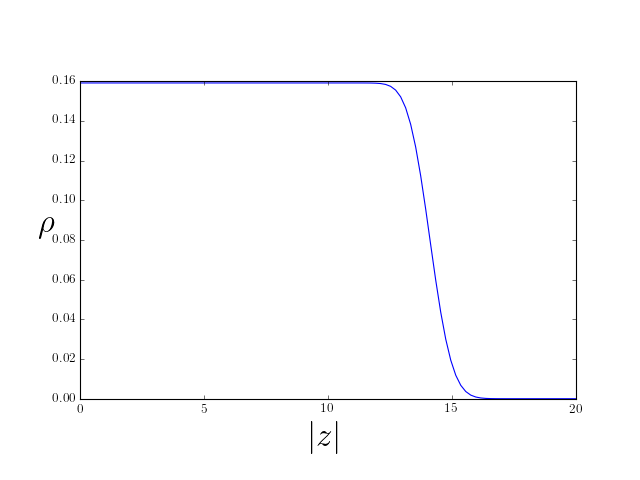
\includegraphics{../LLLdensity.png}

}

\caption{Density of particles in the LLL for \(N=100\)}

\end{figure}%

At small \(\left\|z\right\|\), we can approximate the sum in
\(\eqref{many_LLLdensity}\) by extending the upper limit to \(\infty\),
and we have \(\rho_1\to \frac{1}{2\pi}\). In fact, the density is fixed
at this value until we reach \(\sim\sqrt{2N}\), at which point the
density falls to zero on the scale of the magnetic length.

Thus, with the potential \(\eqref{many_HarmonicRound}\), the filled LLL
is described by a circular droplet of fixed density
\(\rho_1 = 1/(2\pi)\), consistent with one state per flux quantum, which
is the known degeneracy of the LLL. This picture is in fact quite
general: changing the confining potential would cause the droplet to
deform, but the density to remain constant (on the macroscopic scale).

\section{The Laughlin Wavefunction}\label{the-laughlin-wavefunction}

The theory of the fractional quantum Hall effect begins with Robert
Laughlin's famous wavefunction \{\% cite Laughlin:1983aa \%\}
generalizing \(\eqref{many_nu1}\) \[
\Psi_m(z_1,\ldots, z_N) = \prod_{j<k}^N (z_j-z_k)^{m} \exp\left(-\frac{1}{4}\sum_{j=1}^N\left|z_j\right|^2\right).
\label{many_nu}
\] For this wavefunction to describe fermions, \(m\) must be odd. Even
\(m\) describes bosons. I want to emphasize first that despite the
superficial similarity of \(\eqref{many_nu1}\) and \(\eqref{many_nu}\),
they are very different beasts. While \(\eqref{many_nu1}\) is an
(antisymmetric) product state \(\eqref{many_nu}\) is not, and indeed its
expansion in product states is not known in general. Furthermore, the
excitations formed by modifying this state have remarkable properties.
As the abstract to Laughlin's paper puts it:

\begin{quote}
This Letter presents variational ground-state and excited-state wave
functions which describe the condensation of a two-dimensional electron
gas into a new state of matter.
\end{quote}

However, we'll see that the \(m=1\) an \(m>1\) cases do have some common
features. First, we should try and explain where these wavefunctions
came from. Conceptually, the simplest case to discuss is that of
\emph{bosons} interacting via the repulsive potential \[
H_{\text{int}} = g\sum_{j<k}\delta(\br_j-\br_k),\qquad g>0
\label{many_delta}
\] The Laughlin state \(\eqref{many_nu}\) with \(m=2\) has zero
interaction energy. In fact, any state with zero interaction energy must
have \(\Psi_2(z_1,\ldots, z_N)\) as a factor. But if a wavefunction has
a higher degree, then in the presence of the potential
\(\eqref{many_HarmonicProject}\) it will have a higher energy than
\(\Psi_2(z_1,\ldots, z_N)\). Thus \(\Psi_2(z_1,\ldots, z_N)\) is the
ground state.

Laughlin argued that for electrons with Coulomb interaction
\(\Psi_{m}(z_1,\ldots, z_N)\) with \(m\) odd is a good variational
wavefunction. The fact that \((z_j-z_k)\) appears in a power higher than
one means that the particles tend to stay away from each other more than
in the \(m=1\) state, thus lowering their interaction.

To get more precise information about the behaviour of wavefunctions,
Laughlin introduced a powerful analogy between the probability
distribution \(\lvert\Psi_m(z_1,\ldots, z_N)\rvert^2\) of the particles,
and the Boltzmann distribution of particles in a classical 2D plasma.
Before doing that, it's useful to actually `look' at a typical
configuration of particles.

\begin{figure}[H]

{\centering 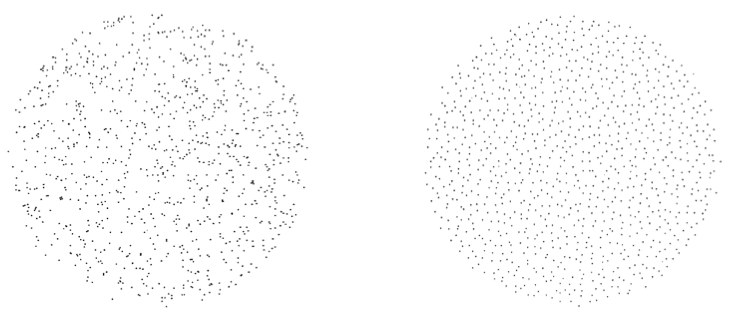
\includegraphics{../assets/LaughlinMonteCarlo.png}

}

\caption{Comparison of Monte Carlo samples from an uncorrelated
(uniform) distrubution of points (left) vs.~the Laughlin probability
distribution \(\lvert\Psi_3(z_1,\ldots z_N)\rvert^2\) (right).}

\end{figure}%

The striking feature of the right hand picture is the \emph{uniformity}
of the particle distribution, in contrast with the sample of
uncorrelated particles on the left. The plasma analogy helps us to
understand this, and a lot more.

\section{The Plasma Analogy}\label{the-plasma-analogy}

The Coulomb potential satisfies \[
\nabla^2 V = -q\delta(\br).
\] In 2D the solution describing a point charge is \[
V_\text{point}(\br) = -\frac{q}{2\pi}\log\,\left|\br\right|,
\] while a constant background charge density \(-\rho_0\) gives rise to
a potential \[
V_\text{bg}(\br) = \frac{\rho_0}{4} \left|\br\right|^2.
\] Thus a system of identical charges in a background charge has an
overall electrostatic energy \[
V(\br_1,\ldots,\br_N) = -\frac{q^2}{2\pi} \sum_{j<k}\log\left|\br_j-\br_k\right| + \frac{q\rho_0}{4}\sum_j \left|\br_j\right|^2.
\] Now we suppose that our plasma is at finite temperature, in which
case the Boltzmann factor giving the (unnormalized) probability of
finding particles at locations \(\br_1, \ldots, \br_N\) is \[
\exp[-\beta V(\brN)] = \left|\Psi_m(\brN)\right|^2,
\] where we set \(\beta q^2/(2\pi) = 2m\) and \(\beta q\rho_0 = 2\).
This observation is Laughlin's plasma analogy. Do bear in mind that we
are not talking about \emph{physical} electrostatic fields -- this is a
mathematical identification of two probability distributions.

Of course, we still have to analyze the statistical mechanical problem,
which is hard to do exactly. Since we are interested in the large \(N\)
limit, we can introduce a continuum charge density \(\rho(\br)\) and
write the electrostatic energy as a functional of \(\rho(\br)\) as \[
\beta V[\rho] = -m\int d^2\br\, d^2\br'\, \rho(\br)\log\left|\br-\br'\right|\rho(\br') + \frac{1}{2}\int d^2\br\, \left|\br\right|^2\rho(\br).\
\]

\begin{quote}
Show that minimizing the energy with respect to \(\rho(\br)\) --
corresponding to finding the most likely configuration -- leads to the
condition \[
-2m\int d^2\br'\, \log\left|\br-\br'\right|\rho(\br') + \frac{1}{2}\left|\br\right|^2 = 0.
\]
\end{quote}

\begin{quote}
Show that applying \(\nabla^2\) to both sides gives \[
\rho(\br) = \frac{1}{2\pi m}.
\]
\end{quote}

On the basis of this approximation, we conclude that the density is
fixed at \(1/m\) of the value we found for the \(m=1\) case, which seems
reasonable. The result applies where the density is non-zero, so we get
a uniform droplet as before, this time of radius \(\sqrt{2Nm}\). \(1/m\)
is called the \textbf{filling fraction} of the state.

Although we ignored the effect of summing over all configuration of the
particles in the partition function (i.e.~we ignored the contribution of
entropy to the free energy), it turns out that this effect can be
ignored in the large \(N\) limit.

\begin{quote}
One odd thing about the above calculation is that if the charge density
is uniform, how does the droplet know where to sit? The location of the
origin is obviously dictated by the minimum of the quadratic term in the
energy, but we could have located that anywhere in the plane and still
had a uniform charge density. Cast your mind back to the old problem of
a mass undergoing simple harmonic motion through a hole in the
earth\ldots{}
\end{quote}



\section{Fractional Charge}\label{fractional-charge}

Laughlin also suggested wavefunctions to describe excited states of the
system, the simplest being the \textbf{quasihole} wavefunction \[
\Psi_\text{hole}(z_1,\ldots, z_N|Z) = \left(\prod_j (Z-z_j)\right)\Psi_m(z_1,\ldots, z_N).
\] In the case of the \(m=2\) state with the interaction
\(\eqref{many_delta}\) discussed above, it's clear that this state still
has zero interaction energy, although the harmonic potential
\(\eqref{many_HarmonicProject}\) acts upon it non-trivially.

The plasma analogy allows us to see that this state describes a
\textbf{quasiparticle} of fractional charge. The concept of a
quasiparticle is one that we'll meet repeatedly in this course. It
describes a particle-like excitation of a many body system.
\textbf{Phonons} -- quantized lattice vibrations -- are a kind of
quasiparticle that you will have met before. In quantum field theory,
particles themselves are described as quantized excitations of a system
-- fields that pervade spacetime -- so at a \emph{formal} level there is
little difference between the particles of particle physics and the
quasiparticles of condensed matter physics. The \emph{physical}
difference is that in the latter case we know what the background medium
is made of!

Let's see how the plasma picture is modified by the introduction of the
quasihole. The electrostatic energy is now \[
\begin{align}
V(\brN)=&-\frac{q^2}{2\pi m}\sum_j \log\left|\br_j-\mathbf{R}\right|-\frac{q^2}{2\pi} \sum_{j<k}\log\left|\br_j-\br_k\right|\\
 &+ \frac{\rho q_0}{4}\sum_j \left|\br_j\right|^2.
\end{align}
\] This is interpreted as the introduction of a charge \(q/m\) at point
\(\mathbf{R} = (X, Y)\), where \(Z=X+iY\). The charges of the plasma
will screen this charge, leaving a `hole' in the density distribution
amounting to charge \(-q/m\), corresponding to \(-1/m\) real particles.
The quasiholes have fractional charge!

A Monte Carlo simulation of a Laughlin state. You can change the inverse
filling fraction \(m\). The red dot is a quasihole: in fact for clarity
it's 20 quasiholes with an overall charge of \(-20/m\).

This means that the normalization integral is approximated by the
Boltzmann weight corresponding to the interaction of this fractional
charge with the background charge density \[
\int \prod_{j=1}^N d^2z_j\,\left|\Psi_\text{hole}(z_1,\ldots, z_N|Z)\right|^2 \sim\exp\left(\frac{1}{2m}\left|Z\right|^2\right),
\]

\section{Fractional Statistics}\label{fractional-statistics}

Consider the two quasihole wavefunction \[
\Psi_\text{2 hole}(z_1,\ldots, z_N|Z_1,Z_2) = \left(\prod_j (Z_1-z_j)(Z_2-z_j)\right)\Psi_m(z_1,\ldots, z_N).
\label{many_2hole}
\] The probability distribution
\(\vert\Psi_\text{2 hole}(z_1,\ldots, z_N\vert Z_1,Z_2)\rvert^2\)
corresponds to a Coulomb plasma with two \(1/m\) charges at the
positions \(\mathbf{R}_{1,2}\). There is no interaction term between
these two fixed charges, but as we have argued, each is overwhelmingly
likely to be surrounded by region of depleted density amounting to
\(-1/m\) of a particle. The normalization integral is then be given by
the Boltzmann weight corresponding to the interaction of these two
depleted regions \[
\begin{align}
\int \prod_{j=1}^N &d^2z_j\,\lvert\Psi_\text{2 hole}(z_1,\ldots, z_N\vert Z_1,Z_2)\rvert^2\\ &\sim\exp\left(\frac{2}{m}\log\left|Z_1-Z_2\right|+\frac{1}{2m}\left[\left|Z_1\right|^2+\left|Z_2\right|^2\right]\right).
\end{align}
\] If we try to intepret this as the probability density of a two
particle wavefunction, we arrive at \[
\Psi_\text{2 hole}(Z_1,Z_2) \sim \left(Z_1-Z_2\right)^{1/m} \exp\left(\frac{1}{4m}\left[\left|Z_1\right|^2+\left|Z_2\right|^2\right]\right).
\]

For \(m=1\) this is an antisymmetric wavefunction, and may be
interpreted as a pair of fermionic holes. For \(m>1\) the wavefunction
is \emph{multi-valued}, and changes by a phase \(\pi/m\) when \(Z_1\)
and \(Z_2\) are exchanged. The quasiholes are \textbf{anyons}, particles
with fractional statistics intermediate between bosons and fermions.

\chapter{Appendix}\label{appendix}

\section{Sampling from a complex
wavefunction}\label{sampling-from-a-complex-wavefunction}

Suppose we have a complex wavefunction \(\psi(\br,t)\) that solves the
Schrödinger equation

\[
i\frac{\partial\psi}{\partial t} = -\frac{1}{2m}\left(\nabla -iq\mathbf{A}\right)^2 + V(\br)\psi(\br,t).
\]

We can write \(\psi(\br, t) = \exp(R(\br, t) + iS(\br, t))\), where
\(S(\br,t)\) is the phase of the wavefunction and the probability
density is \(\rho=|\psi|^2 = e^{2R}\). With some massaging, we can
arrive at the following equation

\[
\frac{\partial \rho}{\partial t} = \frac{1}{2m}\nabla^2\rho - \nabla\cdot\left(\bv \rho\right)
\]

with \(\bv = \nabla R + \nabla S - q\mathbf{A}\). This is a
\href{https://en.wikipedia.org/wiki/Fokker\%E2\%80\%93Planck_equation}{Fokker--Planck
equation} describing the evolution of a probability distribution
\(\rho\) due to diffusion (with diffusion constant \(D=\frac{1}{2m}\))
together with a \emph{drift velocity} \(\bv\), which depends on the
amplitude, phase, and the vector potential. Although the potential
\(V(\br)\) does not appear in this equation, it determines the functions
\(R\) and \(S\).

We can sample from the probability distribution \(\rho\) by simulating
the stochastic differential equation for the particle's position

\[
d\br_t = \sqrt{\frac{1}{m}}d\mathbf{B}_t + \mathbf{v}dt,
\]

where \(\mathbf{B}_t\) is a Brownian motion. In practical terms, this
means that for a small time step \(\Delta t\) we update the position as

\[
\Delta \br_t = \sqrt{\frac{\Delta t}{m}}(X_i, Y_i)  + \mathbf{v}\Delta t,
\]

where \(X_t\) and \(Y_t\) are sampled from a standard normal
distribution of unit variance: \(X_t, Y_t \sim \mathcal{N}(0,1)\)

Extended to the many body case and applied to the Laughlin wavefunction
\eqref{many_nu} we arrive at the drift \(\mathbf{v}_i\) of particle
\(i\), written in terms of the positions \(\mathbf{r}_i = (x_i, y_i)\)

\[
\mathbf{v}_i = -\frac{1}{2}\mathbf{r}_i + \frac{1}{2} \mathbf{r}_i \times \hat{\mathbf{z}} + m \sum_{j\neq 1} \left(\frac{\mathbf{r}_i - \mathbf{r}_j - (\mathbf{r}_i - \mathbf{r}_j)\times \hat{\mathbf{z}}}{|\mathbf{r}_i-\mathbf{r}_j|^2}\right).
\]

This is what I used for the Monte Carlo simulation of the Laughlin
state.

\phantomsection\label{refs}
\begin{CSLReferences}{1}{0}
\bibitem[\citeproctext]{ref-girvin2002quantum}
Girvin, Steven M. 2002. {``The Quantum Hall Effect: Novel Excitations
and Broken Symmetries.''} In \emph{Aspects Topologiques de La Physique
En Basse Dimension. Topological Aspects of Low Dimensional Systems:
Session LXIX. 7--31 July 1998}, 53--175. Springer.

\bibitem[\citeproctext]{ref-stone1992quantum}
Stone, Michael. 1992. \emph{Quantum Hall Effect}. World Scientific.

\end{CSLReferences}




\end{document}
